\section{Adaptor}

Facilitating easy communication between MANOs is an important aspect of scramble. 
Adaptor is a component that enables communication between MANOs by wrapping the REST APIs of MANOs in python code.\\

Python MANO Wrappers (PMW) is a uniform python wrapper library for various implementations of NFV Management and Network Orchestration (MANO) REST APIs. 
PMW is intended to ease the communication between python and MANO by providing a unified, convenient and standards oriented access to MANO API.\\

To achieve this, PMW follows the conventions from the ETSI GS NFV-SOL 005 (SOL005) RESTful protocols specification. 
This makes it easy to follow and the developers can use similar processes when communicating with a variety of MANO implementations.\\

PMW is easy to install, use and well documented. 
Code usage examples are available along with the detailed documentation at the following link \url{https://python-mano-wrappers.readthedocs.io/en/adaptor/}. \\

PMW is planned and released as an independent library. 
In scramble, PWM helps in inter communication of different instances of MANO, thereby creating opportunity for more advanced feature set, for example, hierarchical scaling. 
Operations such as on-boarding of NSD and VNFD, instantiation and termination of NS can be performed with ease.

\subsection{Architecture \& Work flow}
Standards based approach is a fundamental design principle behind PMW's design. 
A Common interface template is defined in compliance with ETSI SOL005 which contains the blueprint for all the methods mentioned in the standards. 
These methods are divided into different sections as per ETSI SOL005 into the following:

\begin{itemize}
	\item \textbf{auth: }Authorization API
	\item \textbf{nsd: }NSD Management API
	\item \textbf{nsfm: }NS Fault Management API
	\item \textbf{nslcm: }Lifecycle Management API
	\item \textbf{nspm: }NS Performance Management API
	\item \textbf{vnfpkgm: }VNF Package Management API
\end{itemize} 

In the figure \ref{fig:wrapperarch}, a high level architecture of PWM is shown. 
As part of the scramble project, support for Open Source MANO (OSM), Sonata and Pishahang are implemented based on the common interface provided by PWM. 
Wrappers also support additional functionalities of Pishahang, which is an extension of Sonata. 

In the figures \ref{fig:osmclassdiagram} and \ref{fig:pishahangclassdiagram}, the class diagram of OSM, Sonata and Pishahang PWM implementation is shown respectively. Note the additional "Admin" functionalities supported by PWM for both OSM and Sonata, these are individual non-standard APIs of the respective MANOs. In the figure \ref{fig:pishahangclassdiagram}, support for Pishahang specific APIs are also implemented along with the database APIs which are part of pg-scramble.

\begin{figure}
	\centering
	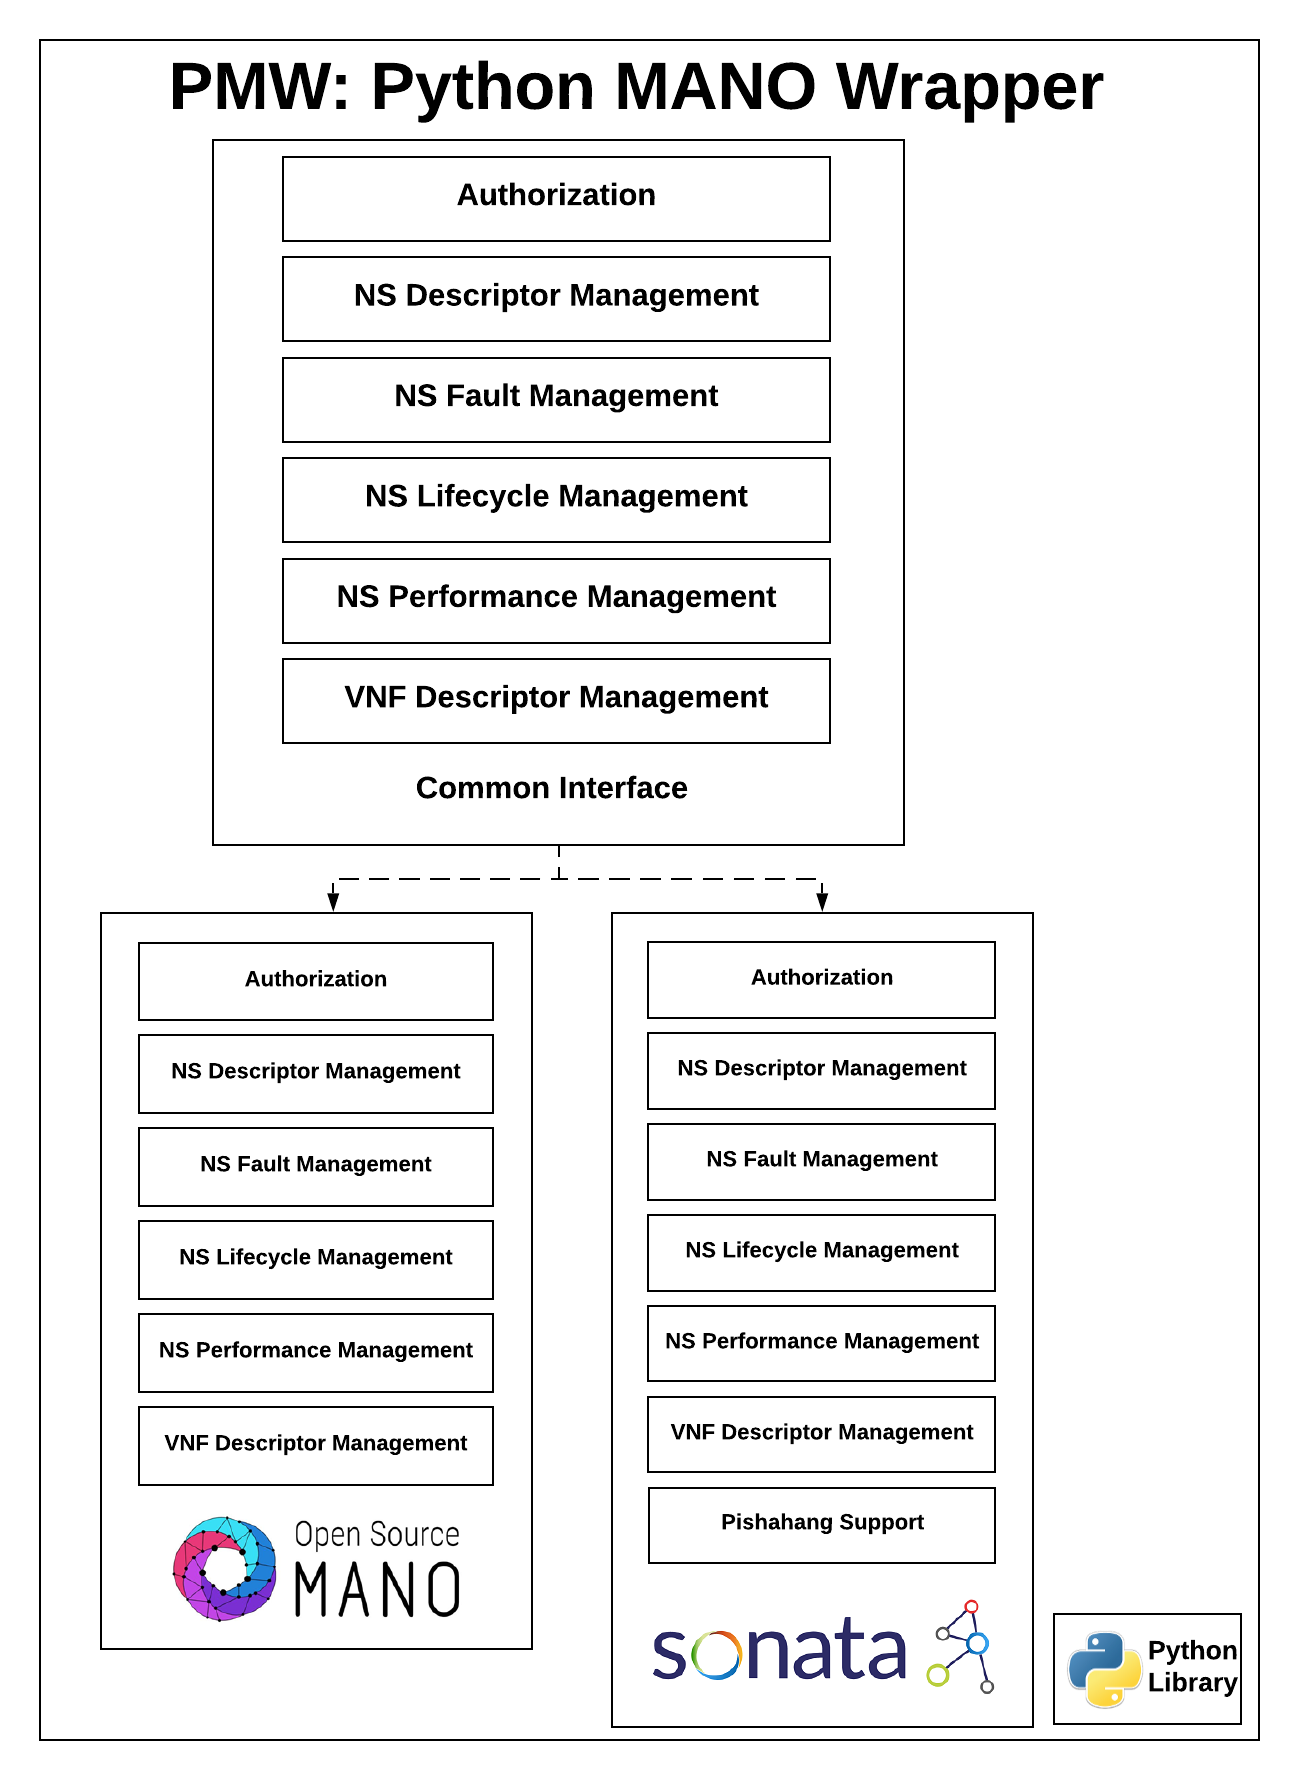
\includegraphics[width=1\linewidth]{figures/WrapperArch}
	\caption{PWM high level architecture}
	\label{fig:wrapperarch}
\end{figure}

\begin{figure}
	\centering
	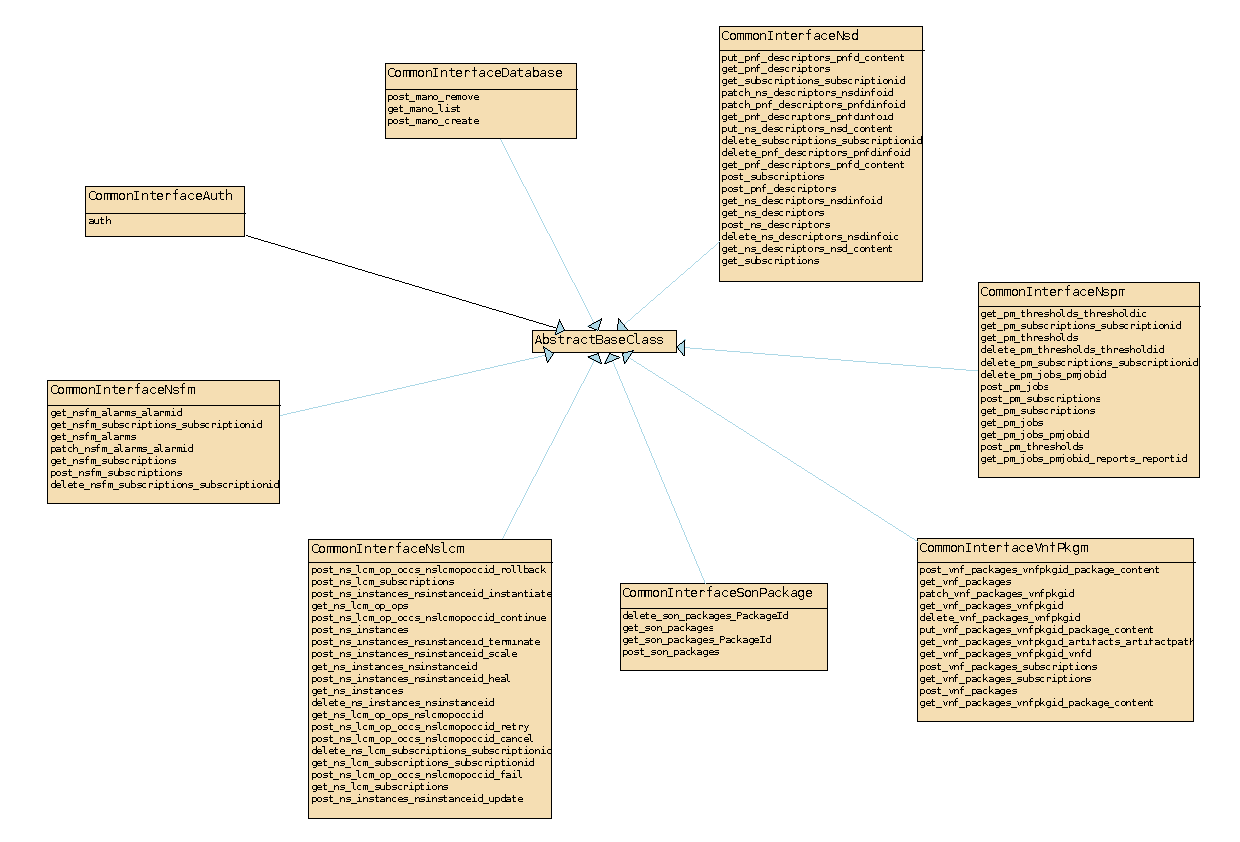
\includegraphics[width=1\linewidth]{figures/common_interface_class_diagram}
	\caption{CommonInterface Abstract Base Classes defined in PWM}
	\label{fig:commonclassdiagram}
\end{figure}

\begin{figure}
	\centering
	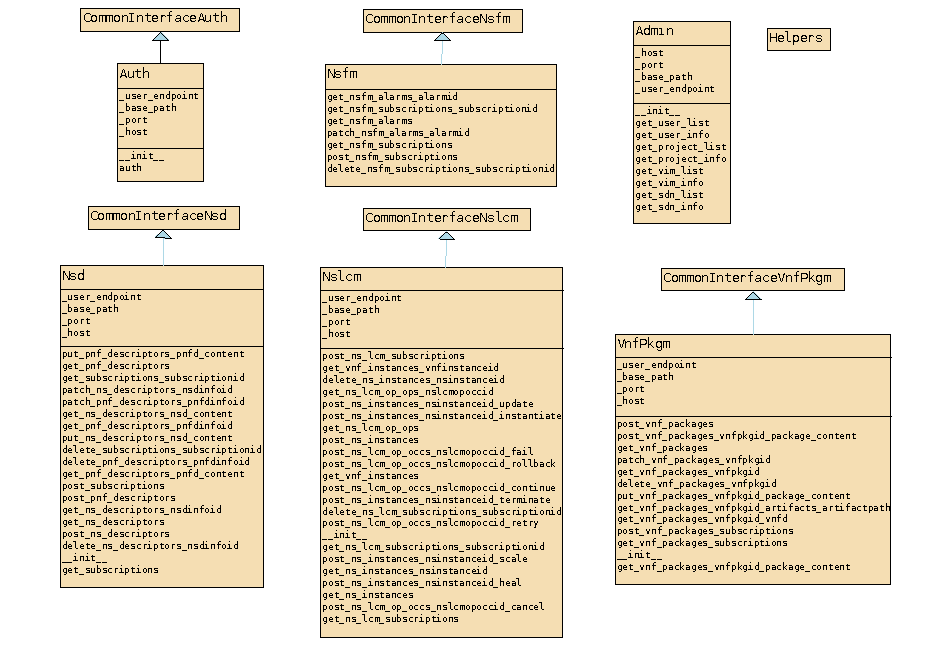
\includegraphics[width=1\linewidth]{figures/osm_class_diagram}
	\caption{OSM Wrappers implemented based on the CommonInterface base classes}
	\label{fig:osmclassdiagram}
\end{figure}

\begin{figure}
	\centering
	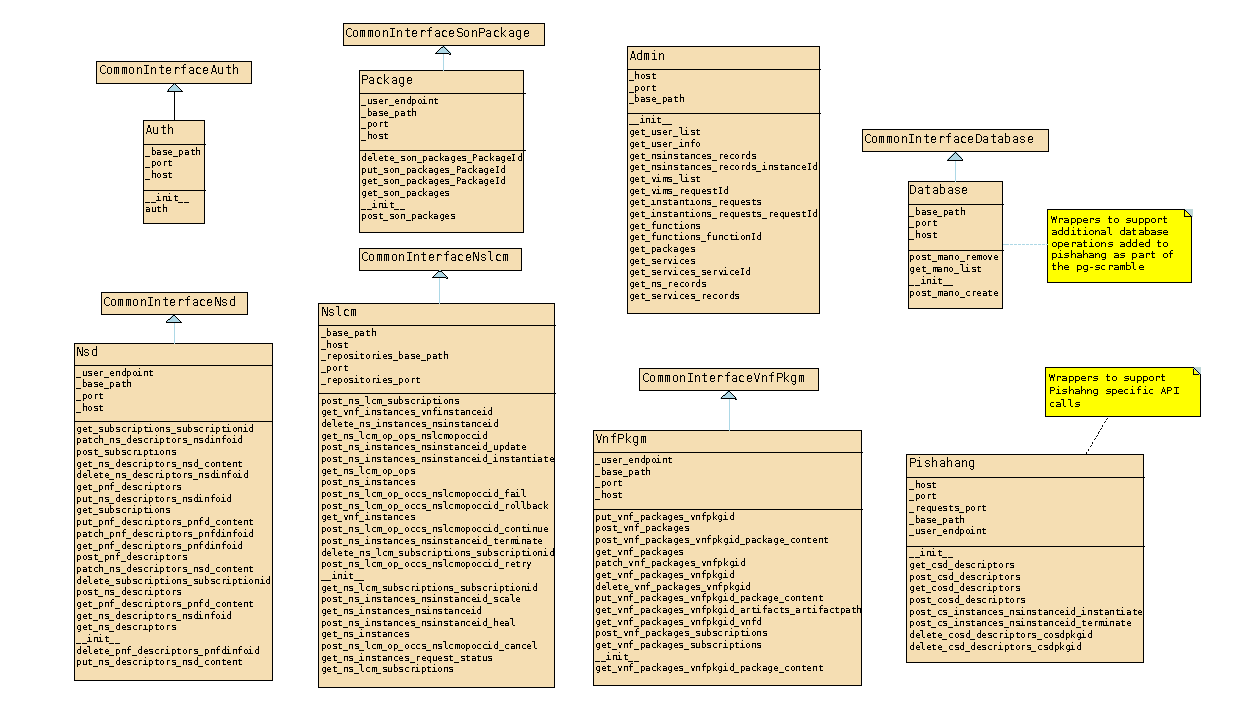
\includegraphics[width=1\linewidth]{figures/pishahang_class_diagram}
	\caption{Sonata and Pishahang Wrappers implemented based on the CommonInterface base classes}
	\label{fig:pishahangclassdiagram}
\end{figure}


\subsection{Installation and usage}

PWM can be installed using pip by using this command \texttt{pip install python-mano-wrappers}. 

A simple script to get started with PWM is shown in the Listing \ref{lis:simpleauth}, here, the wrappers are imported and a client object is created according to the MANO type. 
Currently supported are OSM and Sonata. 
Such a client object can be used to make REST calls relevant to the MANO type. 
An example usage to retrieve all the network service descriptors of OSM can be seen from the listing \ref{lis:osmnsd}, here, the OSMClient module is used to first fetch an auth token and further using the auth token to fetch the relevant information, in this case NSD descriptors.


\begin{lstlisting}[caption=Simple wrapper code to fetch token, label=lis:simpleauth]
import wrappers

username = "admin"
password = "admin"
mano = "osm"
# mano = "sonata"
host = "osmmanodemo.com"

if mano == "osm":
	_client = wrappers.OSMClient.Auth(host)
elif mano == "sonata":
	_client = wrappers.SONATAClient.Auth(host)

response = _client.auth(
							username=username, password=password)

print(response)

\end{lstlisting}

\begin{lstlisting}[caption=Code to fetch all NSDs in OSM, label=lis:osmnsd]
import wrappers

osm_nsd = wrappers.OSMClient.Nsd(HOST_URL)
osm_auth = wrappers.OSMClient.Auth(HOST_URL)

_token = json.loads(osm_auth.auth(
									username=USERNAME,
									password=PASSWORD))

_token = json.loads(_token["data"])

response = json.loads(osm_nsd.get_ns_descriptors(
											token=_token["id"]))
response = json.loads(response["data"])
\end{lstlisting}

\subsection{Challenges}

Implementing such a python wrapper for a REST API is straight forward from the implementation perspective. 
However, the challenges that we faced are when identifying the required functional documentation from the respective MANOs. 
OSM and Sonata do not yet fully support the ETSI suggested endpoints and this combined with the lack of unified documentation, made it difficult in the beginning to decide on the scope of supported functionalities.\\
  

\subsection{Future work}

PWM is built with easy maintainability and feature addition in mind. 
PWM makes it easy to add support for other MANOs. 
We expect MANO developers to use the common interface that we have suggested to add support to their REST APIs in python.

 
